% CVPR 2023 Paper Template
% based on the CVPR template provided by Ming-Ming Cheng (https://github.com/MCG-NKU/CVPR_Template)
% modified and extended by Stefan Roth (stefan.roth@NOSPAMtu-darmstadt.de)

\documentclass[10pt,twocolumn,letterpaper]{article}

%%%%%%%%% PAPER TYPE  - PLEASE UPDATE FOR FINAL VERSION
\usepackage[review]{cvpr}      % To produce the REVIEW version
%\usepackage{cvpr}              % To produce the CAMERA-READY version
%\usepackage[pagenumbers]{cvpr} % To force page numbers, e.g. for an arXiv version

% Include other packages here, before hyperref.
\usepackage{graphicx}
\usepackage{amsmath}
\usepackage{amssymb}
\usepackage{booktabs} 
\usepackage{enumitem}
\usepackage{array}
\newcolumntype{P}[1]{>{\centering\arraybackslash}p{#1}}

% It is strongly recommended to use hyperref, especially for the review version.
% hyperref with option pagebackref eases the reviewers' job.
% Please disable hyperref *only* if you encounter grave issues, e.g. with the
% file validation for the camera-ready version.
%
% If you comment hyperref and then uncomment it, you should delete
% ReviewTempalte.aux before re-running LaTeX.
% (Or just hit 'q' on the first LaTeX run, let it finish, and you
%  should be clear).
\usepackage[pagebackref,breaklinks,colorlinks]{hyperref}


% Support for easy cross-referencing
\usepackage[capitalize]{cleveref}
\crefname{section}{Sec.}{Secs.}
\Crefname{section}{Section}{Sections}
\Crefname{table}{Table}{Tables}
\crefname{table}{Tab.}{Tabs.}


%%%%%%%%% PAPER ID  - PLEASE UPDATE
\def\cvprPaperID{*****} % *** Enter the CVPR Paper ID here
\def\confName{CVPR}
\def\confYear{2023}


\begin{document}

%%%%%%%%% TITLE - PLEASE UPDATE
\title{Analysis and Further Development of ReforesTree}

\author{Klim Troyan\\
ETH Zürich\\
Zürich, Switzerland\\
\and
Silviu Nastasescu\\
\and
Dominic Wong\\
}
\maketitle

\begin{abstract}
    ReforesTree is designed to be a benchmark dataset of forest carbon stock that would encourage scalable financing schemes to protect the forests. To avoid the expensive and subjective manually labelled trees, the authors leverage the recent advancements of AI and propose a fully automatic data processing pipeline. Furthermore, a baseline CNN is implemented to showcase its superiority over models trained on satellite data when forecasting the carbon stock on small-scale, tropical agroforestry sites. This paper will thoroughly present their data, go through every step in the pipeline, reproduce their experiments with the baseline CNN, and compare the expected vs actual results.
\end{abstract}

%%%%%%%%% BODY TEXT
\section{Introduction}
\label{sec:intro}
The degradation of the natural world is unprecedented in human history and a vital driver of the climate crisis. Forest biomass is a crucial influence on future climate.

The world's forest cover has decreased by 361 million ha since 2000, primarily in tropical regions. This raises atmospheric carbon levels and makes up to 18\% of all anthropogenic emissions worldwide. 80\% of land-based biodiversity also has its habitat in forests, particularly tropical forests, and forest ecosystems are under severe pressure due to the risk and frequency of extreme weather.

The carbon offset market is expected to grow by a factor of 100 until 2050 due to high demand and available capital. The main issue is the limited supply of offsetting projects, as forest owners lack upfront capital and market access.\textbf{}

Current manual forest carbon stock inventory methods lead to substantial overestimation of the carbon stock. Recent investigations (Badgley et al. 2021; West et al. 2020) have shown that overestimations in forestry carbon offsetting projects were up to 29\% of the offsets analyzed, totalling up to 30 million tones of CO2e and worth approximately 410 million dollars, resulting in distrust in forest financing. Thus, higher quality and transparent protocols of monitoring, verification and reporting (MVR) are needed.

Several people have developed remote sensing technologies to automate parts of the certification process of forestry carbon offsetting projects (Narine, Popescu, and Malambo, 2020; Dao et al., 2019). Most methods use deep learning models and satellite data because of the recent advancements in both fields. While this approach works well in open-canopy scenarios, it struggles in closed-canopy, so better-quality data is needed. Aerial images from drones would be cheap enough and more suitable for dense forests, but no such datasets are available.

ReforesTree addresses this issue and creates the first dataset of this kind. Furthermore, they develop an end-to-end baseline regression model for carbon stock estimation using individual tree images that outperforms satellite imagery and accurately estimates forest carbon stock within official carbon offsetting certification standards.

\section{Dataset}

The ReforesTree dataset has two main parts:
\begin{itemize}
    \item Six RGB drone images of agro-forestry sites in Ecuador.
    \item 4663 manually collected field data for trees in the six sites. The original paper wrongly specifies 200 fewer trees.
\end{itemize}

The principal field data features are the diameter at breast height (DBH), plantation year, site ID, species, latitude, longitude, and height. The aboveground biomass (AGB), species group, and carbon stock are computed from these values. We also possess the binary tree group (i.e., is the tree a banana tree or not) information. 

There are six types of groups of species: banana, cacao, fruit, citrus, timber, and other. Table \ref{tab:species_distribution} shows the distribution of these species over the six sites. This distribution is present in the paper and thesis. Still, in the latter, the third site is moved to the bottom of the table, and its number of species is larger by one, artificially making the total number of species larger by one. There is no clue how the authors made this mistake.

One thing that is not visible in this table is the class imbalance. From the total number of trees, 44\% are cacao, 32\% banana, 16\% fruit, 3\% timber, 1.5\% citrus, 3.5\% other.

\subsection{Formulas for AGB and carbon stock}\label{agb-cs-subsec}
To compute the AGB values, published allometric equations for tropical agroforestry were used. The authors unwillingly forgot to specify the formula for other, used its equation for fruits, and did not mention that fruits with citrus have the same equation. To realize these three mistakes, we needed to ask the authors for the master thesis on which the paper was written. We checked the referenced articles in the thesis for the formulas, and all five were correct there. We specify them below.

\begin{equation}
AGB_{musacea} = 0.03 * DBH ^ {2.13}
\end{equation}
\begin{equation}
AGB_{cacao} = 0.1208 * DBH ^ {1.98}
\end{equation}
\begin{equation}
AGB_{fruit/citrus} = 0.0776 * DBH ^ {2.64}
\end{equation}
\begin{equation}
AGB_{timber} = 21.3 - 6.95 * DBH + 0.74 * DBH ^ {2}
\end{equation}
\begin{equation}
AGB_{other} = 0.1466 * DBH ^ {2.223}
\end{equation}


To calculate the carbon stock (CS), we need to divide the biomass by 2. Both AGB and BGB (belowground biomass) are needed to compute the biomass. Having the first one, the second value needs to be found. Luckily, we can skip this step by using the root-shoot ratio (RSR), the standard for tropical reforestation sites, its value being 22\%. Thus, to get the carbon value, AGB is enough. This thought process is broken down into the formulas below.

\begin{equation}
Biomass = AGB + BGB
\end{equation}
\begin{equation}
RSR = \frac{BGB}{Biomass}
\end{equation}
\begin{equation}
CS = \frac{Biomass}{2} = \frac{AGB}{2 * (1 - RSR)} \approx AGB * 0.64
\end{equation}

For some unknown reason, the authors' CS values are much lower. Their results show that they multiplied the AGB by 0.39 instead of 0.64, and there is no clue why. Luckily, the AGB values respect the correct formulas, and their CNN baseline predicts AGB instead of CS, so there is still hope their final results are accurate. We finally note that focusing on predicting the DBH in order to then predict the AGB (and hence carbon stock) through the allometric equations would have been a fair approach. However, the DBH values in the dataset were often missing or incoherent (see section \ref{data-imput-subsec}) and were too consequently a result of imputation yielding a poor feature. 

\begin{table}
    \begin{center}
        \begin{tabular}{P{1cm} | P{1.5cm} | P{1.8cm}}
             Site ID & No. Trees & \ No. Species\\
             \hline
             1 & 743 & 18\\
             2 & 929 & 22\\
             3 & 846 & 15\\
             4 & 789 & 20\\
             5 & 484 & 12\\
             6 & 872 & 14\\
             \hline
             Total & 4663 & 27
        \end{tabular}
        \caption{\label{tab:species_distribution}
        Species distribution over the six sites}
    \end{center}
\end{table}

\section{Methods}
\label{sec:method}
In this section, we will present the pipeline described by the authors. First, the field data needs to be clean. Thus, it is necessary to use outlier detection and imputation. Then the trees in the large drone images will be detected. There are two possible methods: manual annotations and automatic detection. While the second one scales, it is far from perfect, as the results will reveal. When the trees are detected, they need to be matched with the field data. Finally, the trees go through a baseline CNN to predict the AGB. Note that we can predict either AGB or carbon stock because the other can be computed by multiplying with a constant.

%-------------------------------------------------------------------------
\subsection{Outlier Detection}
Some trees have DBH either too small or too big. Only banana trees were found to have over 50cm in diameter. The Master thesis and the paper specify that they clipped these values to 50cm for eight trees. The dataset has nine such wide trees, so we believe this was a typo. The tiny trees are kept as they are.

\subsection{Data Imputation}\label{data-imput-subsec}
A severe error present in the paper is the distribution of missing DBH values. The authors say that only three species have no DBH values: 23 limon (citrus), one balsa (timber), and one variable (other). As correctly specified in the thesis, these species miss \textbf{all} DBH values, but the total number of missing diameter values is 2621, so more than 56\%! We hope this was a mistake in the formulation and there was no intent to hide the poor quality of the data.

Another mismatch between the paper and thesis is the imputation method. The paper said the missing values are filled with the average of the same year and species group trees, whereas the thesis said they used the median. By looking at the imputed field data, the latter is the one used.

%-------------------------------------------------------------------------
\subsection{Manual Data Annotation}
The classic method to extract the trees in images is to do it manually. Its drawbacks are that it is expensive, time-consuming, and subjective. However, supervised learning models need this type of data to be trained.

This process involves drawing a square box around a tree and writing its label. For simplicity, instead of using the six classes, the trees were labelled as either banana or non-banana, as banana trees are easy to recognize. The authors say they manually labelled 324 bounding boxes, but these were not present in the data they provided. We sent an email for these boxes, but they did not answer.

Thus, we did it. To ease our work, we used Roboflow, an online annotation tool. Not only we manually labelled the trees in the areas of interest, but also most of the other trees in the images, being around 8000 trees! We hope these data will be used in the future by people who want to train models for this task. A sample of the annotated images can be seen in Figure 1, with the pink boxes being the banana trees and the red boxes being the non-banana trees.

\begin{figure}
\centering
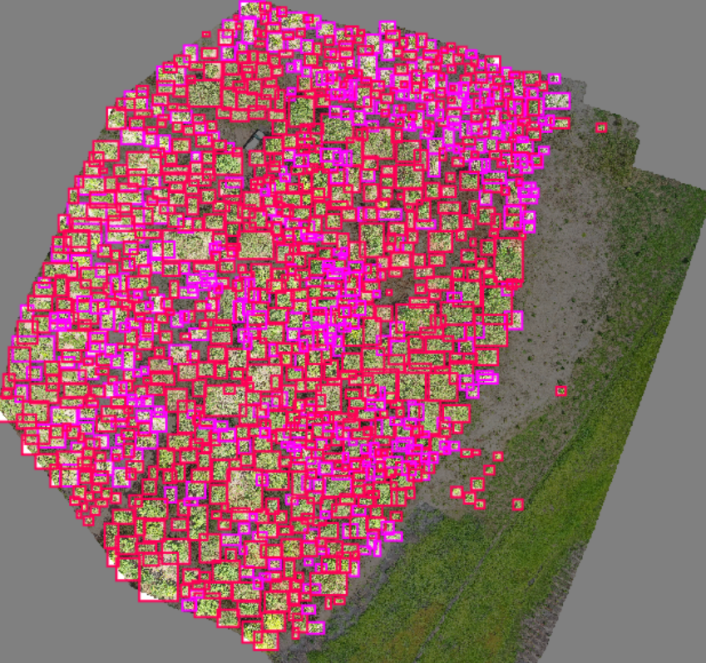
\includegraphics[width=1.\linewidth]{latex/figures/annotations/3.png}  
\caption{Sample of manually annotated images}
\label{annotations}
\end{figure}

%-------------------------------------------------------------------------
\subsection{Tree Crown Detection}
The authors of the ReforesTree dataset use the Deepforest library \cite{weinstein2020deepforest} to detect trees in drone images.
This library contains pre-trained convolutional neural networks for tree crown detection.
The original authors use a pre-trained ResNet model, fine-tuned with hand-labelled annotations of tree crowns in the drone images.
The fine-tuned detection model detects tree crowns without classifying each detection into tree groups or species.

We reproduce the tree crown detection with the fine-tuned model.
This model is publicly available as part of the dataset.
The purpose of reproducing this step in the pipeline is twofold.
First, it allows us to investigate the performance of the detection model.
Second, we obtain the bounding boxes of all the detected trees in the image.
This is not available in the dataset, as the detections not matched to a field measurement are filtered out.

%-------------------------------------------------------------------------
\subsection{Matching Algorithm}
The authors of the ReforesTree dataset use algorithms from optimal transport to match the predicted tree crowns to the field measurements. 
Each field measurement includes the GPS coordinates of the tree.
Each RGB image is associated with a GPS coordinate, as well as longitudinal and latitudinal scales for the height and width of the image.
Thus, the GPS location of each pixel of the image can be calculated.
The relative position of the field measurements and the detected tree crowns is then used by the matching algorithm.
This step of the pipeline is critical due to the large noise in the position of the field measurements.

To investigate this step in the pipeline, we first reproduce the intermediate result of the matching algorithm.
The optimal transport algorithms are implemented in the OneForest library \cite{weinstein2020cross}, which is not open-source. Therefore, we requested the source code from the authors.
We show that the matching algorithm used in the original dataset fails to assign field measurements to the detections accurately.

We investigate the following shortcomings in the original implementation and present some improvements to reduce the number of false matches.
First, we show that a large portion of the field data is assigned to trees outside of the region of interest.
These trees are unlikely to have been surveyed during data collection.
Second, we highlight the issue that the matching algorithm is not constrained by tree species.
This means that, for example, measurements of a banana tree can be assigned to a cacao plant.
Third, we show that some trees are assigned to multiple field measurements.

% ToDo Klim/Dominic, please discuss the additional/redundant/useless features in the final CSV file in a section that you find appropriate. Maybe here? Or section 4.2 Oneforest results? 

%-------------------------------------------------------------------------
\subsection{Complete AGB Prediction Pipeline}\label{agb-pred-subsec}
The data can be obtained either through a \href{https://github.com/gyrrei/ReforesTree}{shared folder} or through the \href{ https://torchgeo.readthedocs.io/en/latest/api/datasets.html#reforestree}{PyTorch Torchgeo datasets library}. The former method provides more data features and details useful for experiments and is hence the one that we mainly used. We start by creating the dataset by sampling individual tree images (zero-padded to same dimensions) obtained from the bounding boxes (within RGB image tiles) to field data matching algorithm, their associated features (e.g., tree group) and the target value. Similarly to the ReforesTree paper, we chose to use the AGB as target value, although DBH or directly carbon stock could have been used given a different quality of data (see section \ref{agb-cs-subsec}). A pre-processing step such as removing outlier values can be performed before the sampling. We then split the dataset into training, validation and test sets. If categorical features such as the (binary) tree group are to be used, they are one-hot encoded when creating the dataset. We create PyTorch data loaders from the datasets to work with mini-batches during training and evaluation. Transforms (e.g., resizing, flips) can be applied to the individual tree images at this step.

The predictive model is defined with an input that depends on whether other features are used in addition to the individual tree images. The output size is $1$ as it is an AGB regression task. The optimizer, criterion and relevant hyper-parameters (e.g., batch size, learning rate and scheduler, number of epochs, etc.) are set. Note that an extensive hyper-parameters search (e.g., Grid search) was not found to be useful. We then proceed with training using the hold-out validation set to evaluate the model through its produced RMSE and MSE loss for every $print\_interval$ number of batches seen. After training is completed, we evaluate the trained model on the hold-out test set and obtain an RMSE score performance. The complete experiments' logs are saved and visualized in \href{https://wandb.ai}{WandB}.

%------------------------------------------------------------------------
\section{Results}
\label{sec:result}

%-------------------------------------------------------------------------
\subsection{Tree Crown Detection with DeepForest}
We reproduce the results of the tree crown detection with DeepForest.
The results are visualized in Figure~\ref{deepforest-detection}.
We see that the fine-tuned model successfully detects a lot of the trees in the RGB image.
In this subsection, we highlight some shortcomings of the current approach.

\begin{figure}
\centering
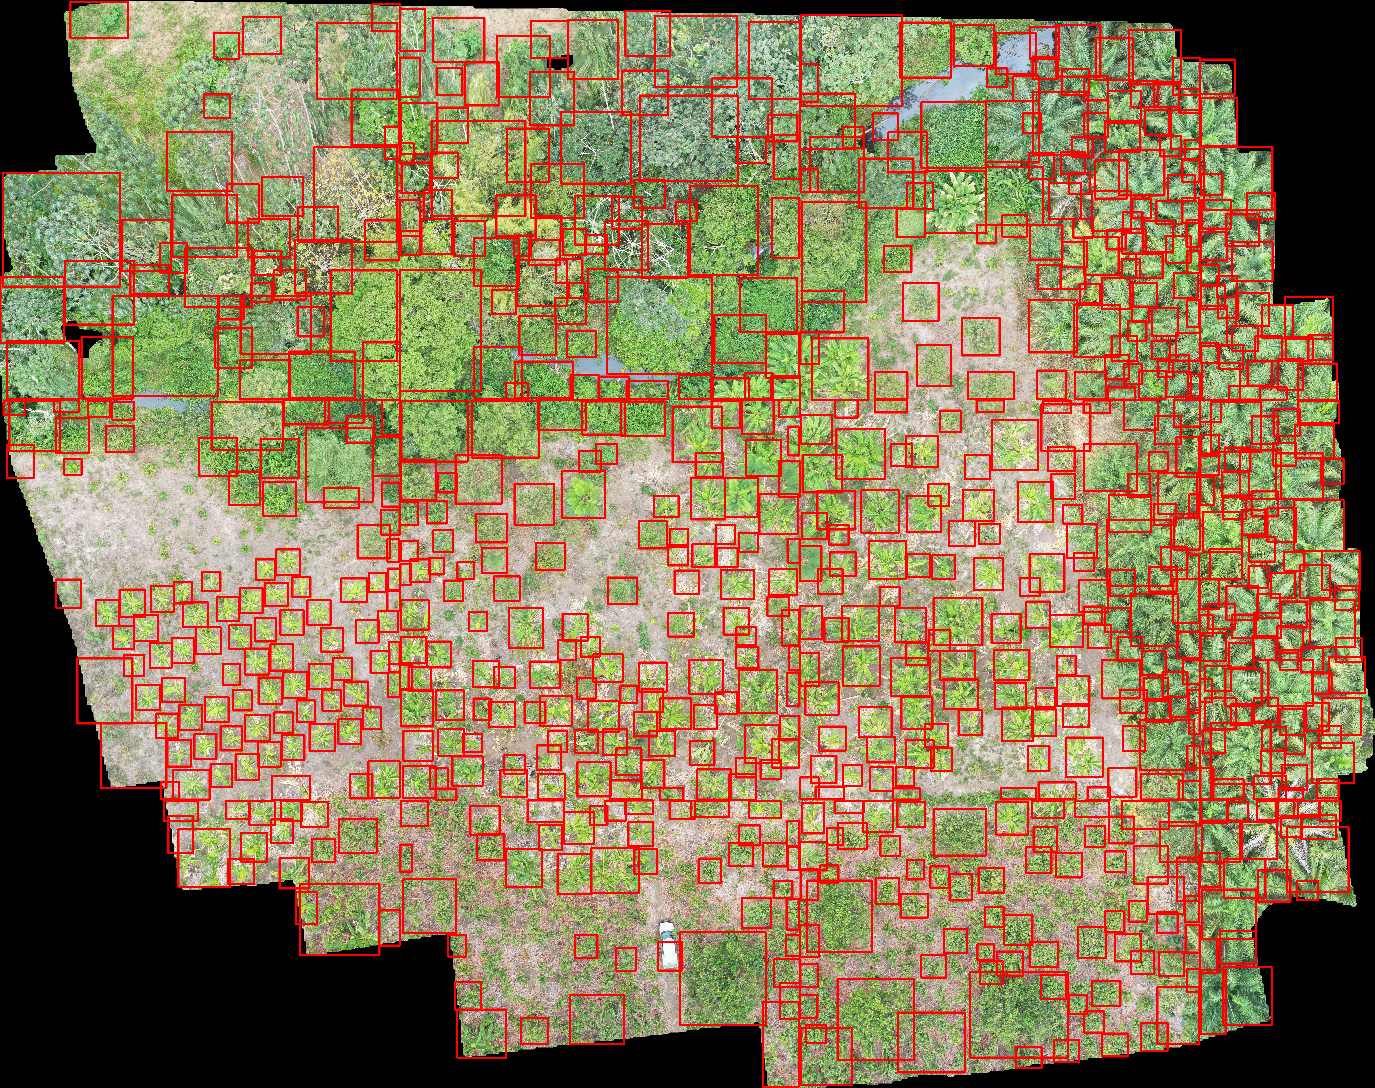
\includegraphics[width=1.\linewidth]{latex/figures/deepforest/Manuel Macias RGB_predicted_boxes_compressed.png}  
\caption{Reproduced tree crown detection with original fine-tuned model}
\label{deepforest-detection}
\end{figure}

First, the model used by the original authors struggles in crowded regions.
As no ground truth bounding boxes are available, we cannot quantitatively evaluate the performance of the detection model.
Instead, we show in Figure~\ref{deepforest-fail} an example where the detection model performs poorly.
Namely, it tends to split a single tree into multiple trees or combines multiple trees into a single detection.

\begin{figure}
\centering
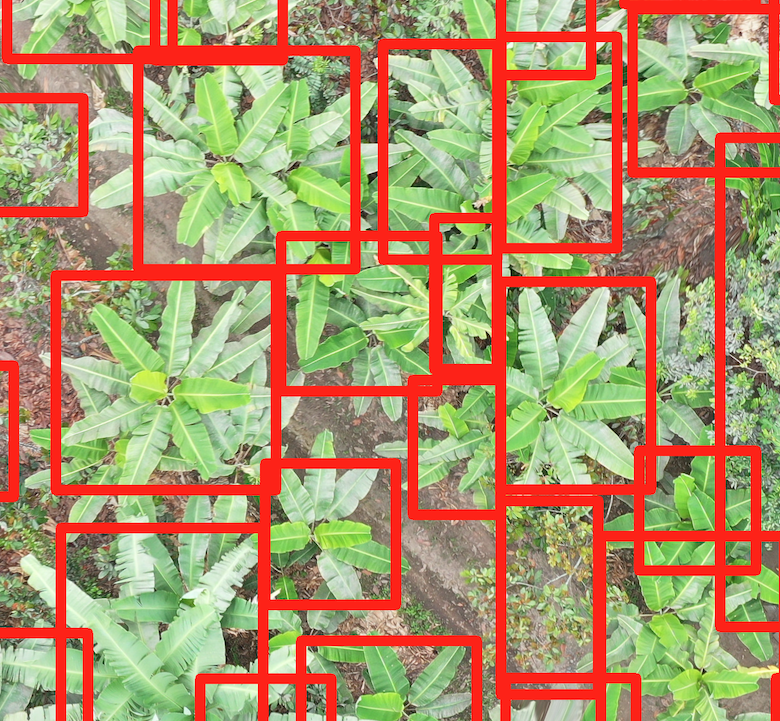
\includegraphics[width=0.9\linewidth]{latex/figures/deepforest/deepforest_fail.png}  
\caption{Original detection model performs poorly in crowded regions}
\label{deepforest-fail}
\end{figure}

The model also fails at detecting small trees or shrubs.
This is an issue in this context because a large portion of the dataset are cacao plants, which are small shrubs in the RGB images.
This affects the data processing pipeline downstream, as it leads to false assignments between detected trees and field measurements.

Finally, the model does not classify the detected trees by their species or group.
We discuss in the next subsection why this is beneficial for data processing and data quality.

%-------------------------------------------------------------------------
\subsection{Matching Algorithm with OneForest}
We reproduced the intermediate results of the original matching algorithm by following the source code of the OneForest Libary.
The results are visualized in Figure~\ref{oneforest-original}.
Each bounding box represents a tree detection and each red cross is the (noisy) GPS location of a field measurement.
The matching is visualized here in white lines.

\begin{figure}
\centering
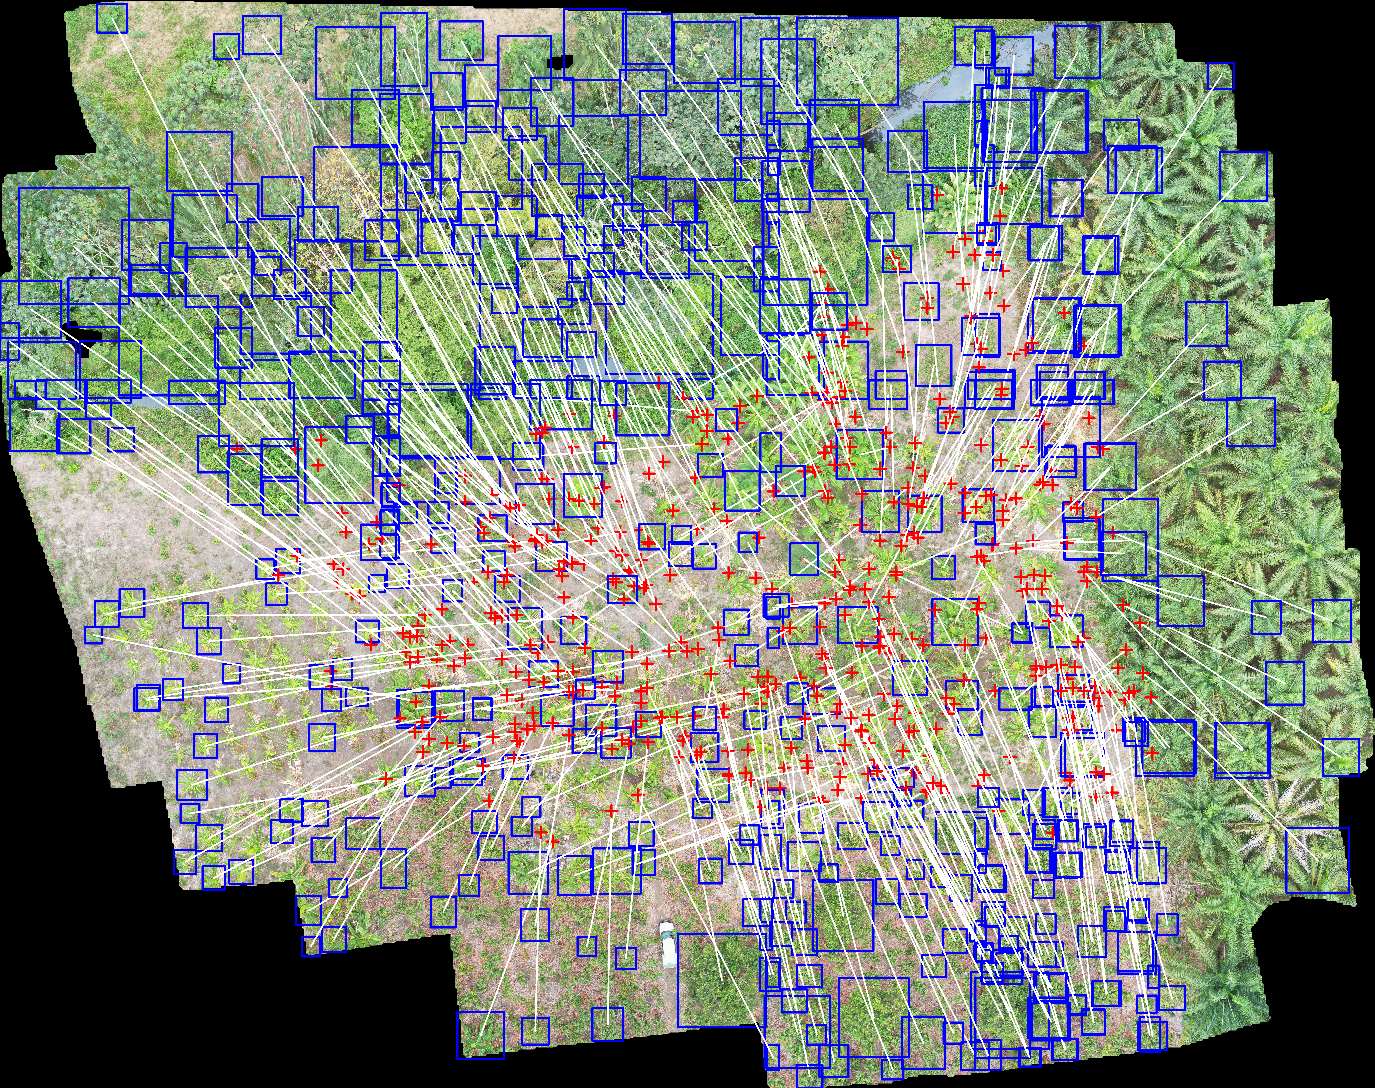
\includegraphics[width=1.\linewidth]{latex/figures/oneforest/Manuel Macias RGB_final_dataset_mappings_compressed.png}  
\caption{Reproduced results of the matching algorithm with OneForest}
\label{oneforest-original}
\end{figure}

In the original implementation, every tree detected in the RGB image is taken into consideration as possible matches for the field data.
The optimal transport algorithm matches the query set (field measurements) to the full range of the target set (tree crown detections).
This leads to a large portion of the field measurement data being matched with trees on the edge of the RGB image, which are not part of the region of interest.
Thus, these are clearly false matches.

The dataset includes polygons that describe the region of interest where the field measurements are taken.
The matching algorithm can be constrained to only trees detected inside this region.
However, the number of trees detected in this region by the CNN is less that the number of field measurements.
The region of interest can be dilated, such that the number of trees within the dilated polygon is equal to the number of measurements.
This unfortunately leads to the same problem described earlier.
The reason is that the number of trees detected within the region is very small.
The polygon must be dilated to such an extreme that trees that are far from the region of interest are also considered by the matching algorithm.
From Figure~\ref{oneforest-with-out-of-site}, we see qualitatively that a large portion of the field data is matched to trees unlikely to be part of the field data.

\begin{figure}
\centering
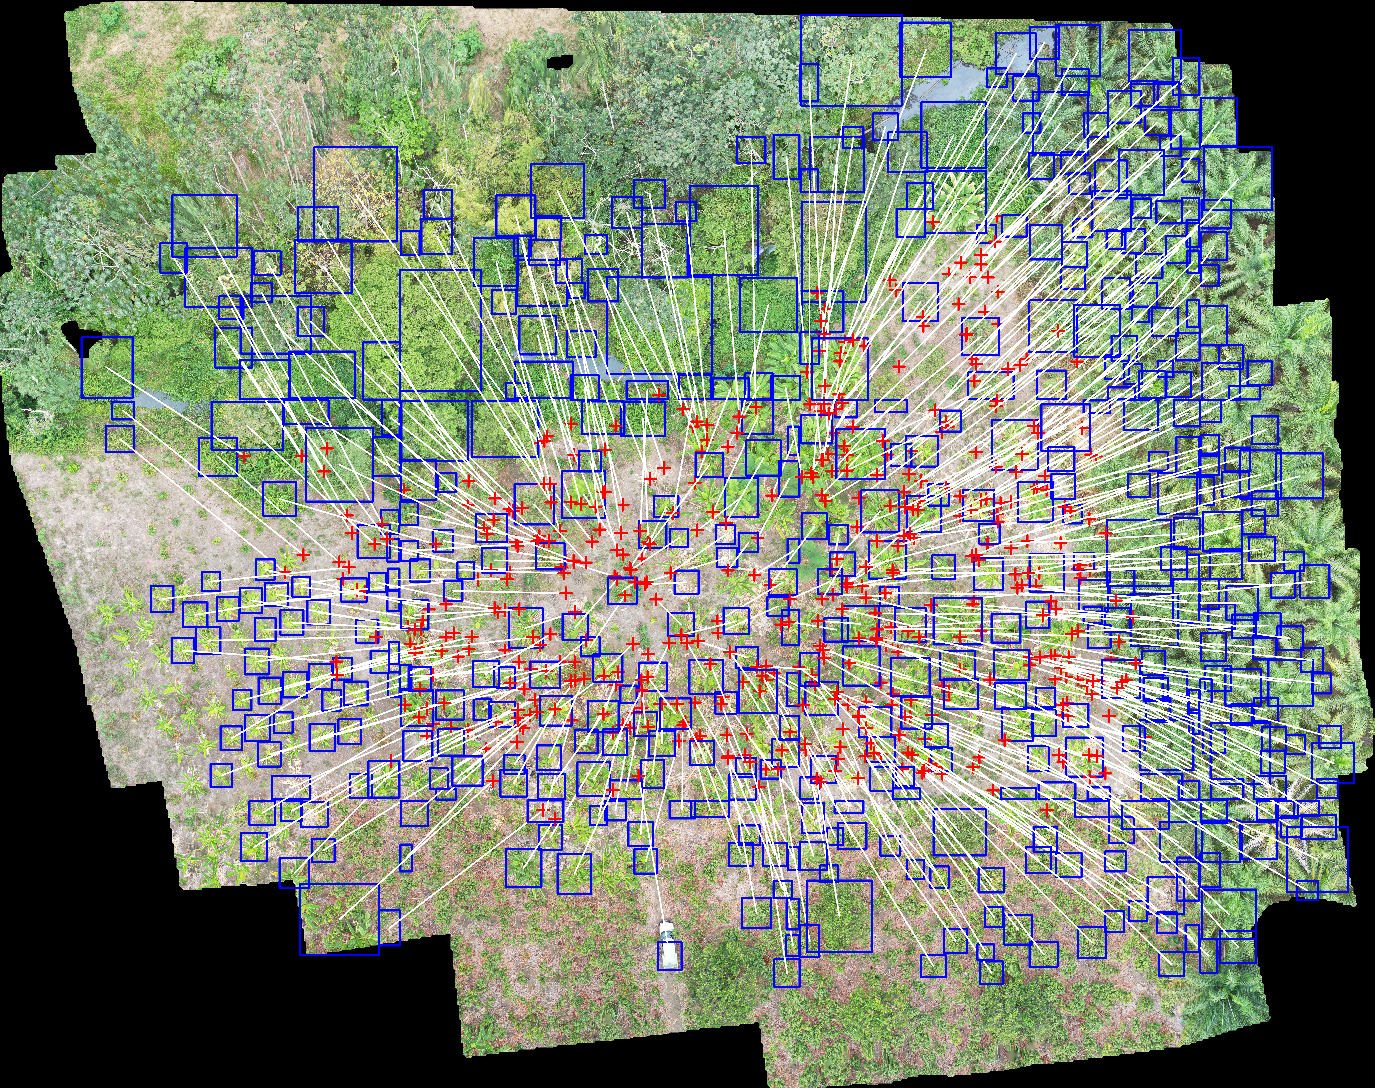
\includegraphics[width=1.\linewidth]{latex/figures/oneforest/filter-out-of-site_with-dilation.png}  
\caption{Constraining the matching algorithm to trees detected within or close to the region of interest}
\label{oneforest-with-out-of-site}
\end{figure}

In Figure~\ref{oneforest-with-out-of-site}, we also notice that the number of matched trees within the region of interest is less than the number of detected trees.
This proves the previous statement that the optimal transport algorithm matches the query set to the full range of the target set.
Thus, this kind of algorithm tends to ignore trees densely packed in the region of interest.

Second, the matching is not constrained by the tree group or species.
This constraint is not possible, as the tree crown detection model does not predict the tree group or species.
This severely decreases data quality, as it leads to measurements being assigned to trees of different species.

This problem can be overcome by training a detection model that also classifies each tree into a species or group.
For matching, the optimal transport algorithms additionally minimize the cross entropy between the predicted species and the species in the field measurement.
Thus, it increases the likelihood of correct matches.

To illustrate this, we match the manually annotated bounding boxes to the field measurements.
The manual annotations include a binary attribute, assigning each annotation to the following groups: "banana" or "non-banana".
The optimal transport algorithm is constrained to take this group into account.
By doing so, we are certain that no trees are assigned measurements from a tree of a different species.
We visualize the matching for the banana tree in Figure~\ref{oneforest-with-tree-group}.
We see qualitatively  that the matches are more ordered and they are close to or within the region of interest.
Furthermore, the matches, represented as white lines in Figure~\ref{oneforest-with-tree-group}, appear to be directed in one direction.
This suggests that the noise in the GPS coordinates has a non-zero mean.
This further supports the idea that such a constrained matching algorithm leads to matches that are more representative of the ground truth.

\begin{figure}
\centering
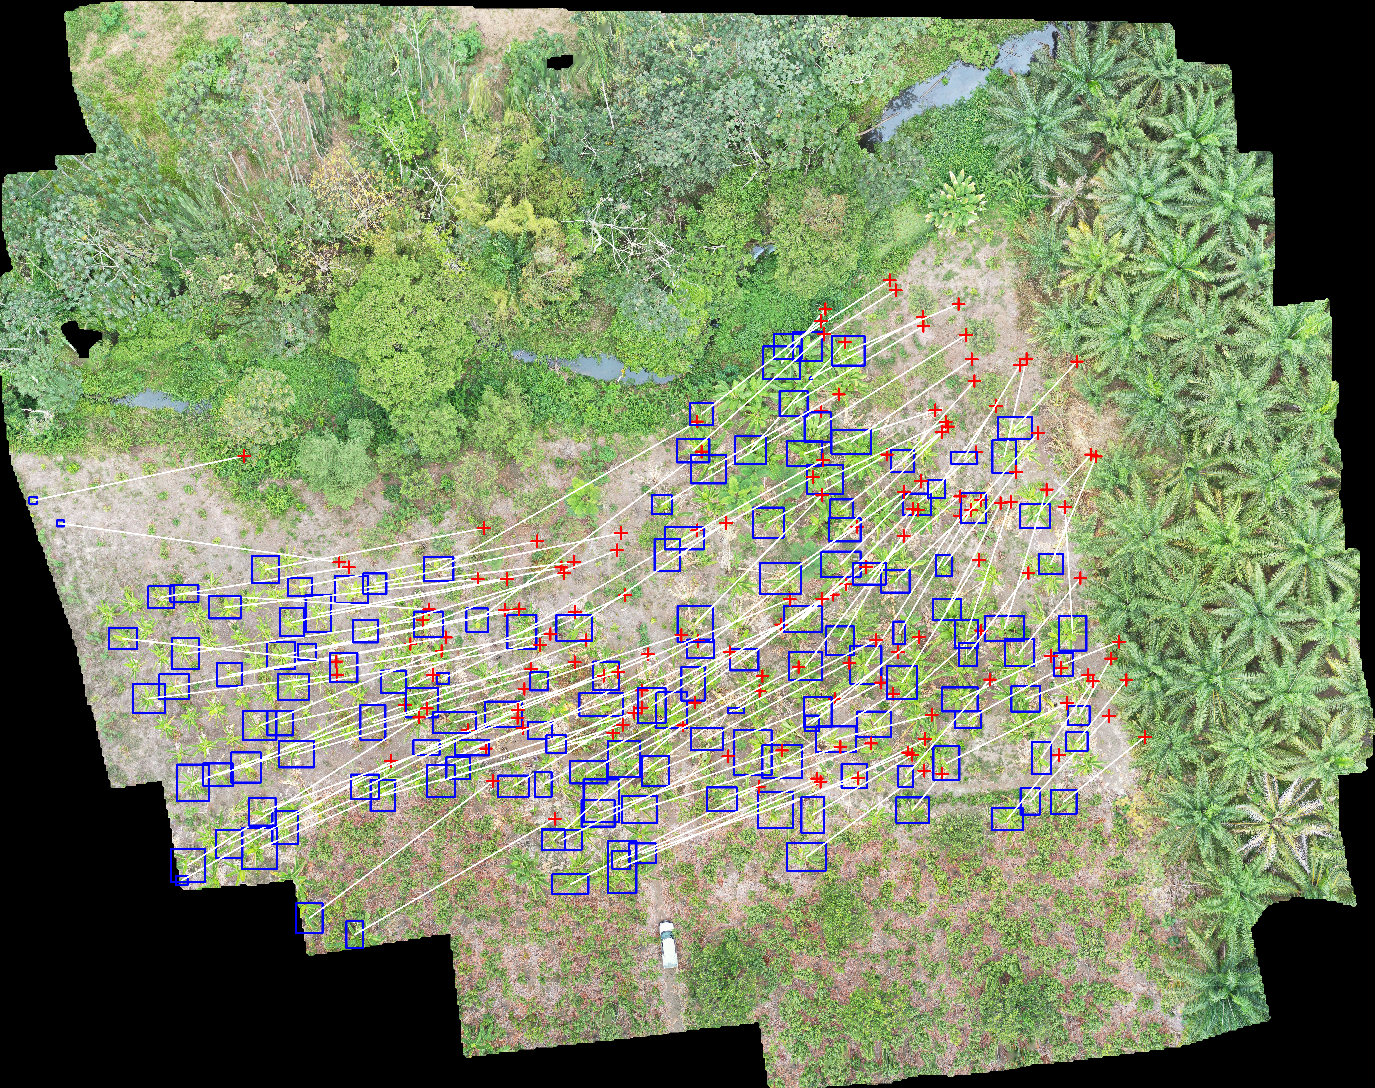
\includegraphics[width=1.\linewidth]{latex/figures/oneforest/matching_with_hand_annotations_banana_compressed.png}  
\caption{Matches for banana trees with the matching algorithm constrained to minimize the cross-entropy of the tree group}
\label{oneforest-with-tree-group}
\end{figure}

Finally, the matching algorithm is not constrained to bijective mappings.
This means that multiple field measurements can be mapped to the same tree.
Indeed, a total of 1572 data points in the final dataset have duplicate bounding boxes.
This suggests that at least 786 data points are matched to the wrong tree, which represents 16.9\% of the final dataset.
Most of these conflicting matches assign measurements of different species to a single tree.
In Table~\ref{tab:conflicting_matches}, we summarize the number of conflicting matches for each tree group.
Evidently, this issue is non-negligible.

\begin{table}
    \begin{center}
        \begin{tabular}{P{1cm} | P{1.5cm} | P{2.5cm}}
             Group & No. Trees & \ Percentage (\%)\\
             \hline
             Banana & 160 & 11\\
             Cacao & 816 & 40\\
             Citrus & 29 & 43\\
             Fruit & 433 & 58\\
             Other & 67 & 42\\
             Timber & 67 & 49\\
             \hline
             Total & 1572 & 34
        \end{tabular}
        \caption{\label{tab:conflicting_matches}
        Number and distribution of conflicting matches between tree detections and field measurements}
    \end{center}
\end{table}

%-------------------------------------------------------------------------
\subsection{AGB Predictions}
Following the complete pipeline described in section \ref{agb-pred-subsec}, we explicit the steps taken and results obtained regarding the reproduction of the ReforesTree paper's baseline predictions result - as they are part of the paper's contributions - as well as our own prediction results and models. 
\subsubsection{Reproducing ReforesTree Paper's Predictions}
After obtaining more detailed information on the experiment settings from the authors, an important part of the work is to manage to reproduce (reasonably) their results. Specifically, an RMSE of $0.1$ could \textbf{not} be achieved by far, despite following the experiment settings exactly as described, and even when using custom datasets whose sole goal is to lower the RMSE score obtained.

To obtain the initial dataset, we (and thus they) sample the individual tree images randomly and balanced with respect to the agro-forestry sites and binary tree group label (i.e., banana or non-banana). Hence, $100$ trees are sampled from each site and for each group, resulting in a total of $1200$ tree samples. Despite it being a much lower number of trees than the complete dataset of $4663$ trees, it is an appropriate choice as there is a strong imbalance across the sites and tree groups. Moreover, it accommodates our lack of high RAM storage. Then, the training, validation and test datasets are obtained by splitting $70-30$ the initial dataset for training-validation, followed by a $90-10$ split for train-test. This yields $756$ trees for training, $360$ trees for validation and $84$ trees for testing. 

The individual tree images were padded with dimensions $800 \times 800$ and then resized to the ResNet18\cite{https://doi.org/10.48550/arxiv.1512.03385} dimensions of $224 \times 224$. The individual tree images are then fed as input to the model for predictions.

The model used is a pre-trained ResNet18 fine-tuned on our dataset. There are essentially two versions (depending on the exact dataset on which it was pre-trained) of pre-trained ResNet18 that can be immediately loaded from the PyTorch Torchivision library, so we performed the experiments with both (without notable differences). We then have the choice to fine-tune all the pre-trained ResNet or use it as backbone by freezing all its layers except the last fully connected layer. Not sure what choice the authors made, we experimented with both (the latter case yielding much lesser parameters to learn and similar predictive performance). Although in the ReforesTree paper, they use a ResNet18 for the baseline, we also performed the experiments with a ResNet50 to see if higher model capacity could help, but no considerable difference in score performance was observed despite being slower to train. No transformation of the input images of the model is performed.

The batch size used across all the experiments was $32$ or $64$ (as authors used). The criterion used is the MSE loss. The optimizer and activation layers were not known, thus we assumed the common Adam\cite{https://doi.org/10.48550/arxiv.1412.6980} optimizer and ReLU\cite{https://doi.org/10.48550/arxiv.1803.08375} activation layers. The learning rate chosen by the authors is $1^{-3}$, hence we used the values of $1^{-i}$, with $i \in \{2, 3, 4, 5\}$ for all the experiments. The number of epochs was always at least $30$ (as per the authors), controlling for no improvement in training if higher than $30$.  

The authors claim to have obtained an RMSE of $0.1$, which is the only value of the only metric shared for their model on the ReforesTree dataset. We naturally assume that they mean it on the test set. The best RMSE we obtained while trying to reproduce their results is $13.0$ on testing and $9.2$ on validation. An RMSE close to $0.1$ could only be obtained on some batches during training. Even using different arbitrary pre- and post-processing techniques with the goal of lowering the RMSE, the RMSE obtained remained far above $0.1$, with the lowest test result of $1.4$ for a very unrepresentative choice of pre-processed samples from the full dataset. For this "extreme" experiment, we removed numerous meaningful outliers and did not select the samples randomly across the dataset by picking ones with the lower AGB values. We can see that the results are relatively far from the $0.1$ RMSE obtained by the authors who also claim that this score performance could be improved fairly easily. They also write that their model basically overfits on the average target value. Considering the large range, (e.g., $\sim 0-200, 0-50$) of the AGB target variable, an RMSE of $0.1$ on a test set of $84$ samples seems difficult to obtain in the current settings and should in fact be considered a great achievement.


\subsubsection{Further AGB Predictions}
While following a similar pipeline for our own predictions, we experimented with different techniques, models and hyper-parameters. Still, we did not consider our results relevant for comparison to the paper's baseline as too far from it. For example, when only removing outliers, the lowest RMSE obtained for testing was $3.4$. Otherwise, the datasets used were the same as that of the previous section for consistency and being able to compare with the paper's prediction pipeline. 

Clearly, for the modeling part, our focus has been on reproducing the results of the ReforesTree paper with goal to then be able to compare our potentially improved models to that used to obtain the same results. However, as discussed in the previous section, we did not succeed and therefore the modeling aspect had less importance improvement-wise. Besides the different setting choices made and described in the previous section while trying to reproduce the ReforesTree paper's prediction results, we built different CNN-based models and explored different common training methods. Using a pre-trained ResNet with fine-tuning showed to yield better results than training a simpler CNN from scratch.

A technique that constantly yielded improvements is to define a multi-input model considering the input tree images and additional features such as the tree group label. In order to do so, we embed the categorical feature in a one-hot vector and concatenate it to the outputted transformed image input passed through the pre-trained ResNet during the forward pass. This supports the model learning by providing meaningful semantics (assuming that the additional features are correct) to the model. We note that the usage of the tree group as an additional feature is reasonable as the tree crown detection model can be trained to predict the tree group at the same time of detecting the trees within the RGB drone images to predictions pipeline. Then, having simply fully connected final layers with ReLU activation functions in-between performed as well as having a more complicated sub-network that did not seem to provide a better representation for prediction than the ResNet.

% ToDo: Klim, don't forget to specify both the RMSE values, namely the one we got by using their method (was it 13?) and the one that we got using only the data with the smallest AGB values to get the best possible RMSE (which was 1.5). The only 0.1 RMSE we were able to get was on some overfitted training batches... --> OK

%------------------------------------------------------------------------
\section{Discussion and Possible Improvements}
\label{sec:discussion}
We believe that field data pre-processing could have been performed better. For instance, the outliers were considered to be the trees with over 50cm diameter, and these values were clipped to 50cm. There is no justification for doing so, considering that all these trees were banana trees planted in the same year as other much narrower trees. The same reasoning can be applied to tiny trees. From a simple look at the data, it can be seen that most trees have DBH between 1.5 and 30 centimetres, with only two trees having below 1cm diameter and 14 above 30cm. Removing these 16 values and letting the imputer find a suitable value seems a more reasonable approach. However, if the data were more extensive and complicated, isolation forests \cite{liu2008isolation} would better find outliers.

Talking about the imputer, there is no problem with their method. However, it would have been better to use the k-nearest neighbors (kNN) \cite{peterson2009k} imputer that uses not only the year and species group but also the species name and height. We implemented it and noticed that most of the values were similar, with larger differences for the underrepresented species, which encourages the idea that kNN would have been preferred.

The issues with the tree crown detection can be easily addressed by training a new tree crown detection model, fine-tuned for this specific use case.
The original model is based on the RetinaNet model \cite{retinanet}.
With recent advances in convolutional neural networks such as YOLO \cite{yolo} and vision transformers \cite{detr}, we expect that there is much room for improvement here.
Our manually annotated data serves as a training and evaluation dataset.

The matching algorithm represents a fragile and critical part of the data processing pipeline.
The reason is that its inputs are noisy GPS data and predicted tree detections.
While we've represented some solutions to improve the accuracy of the matching algorithm, we also show that the problem of the matching algorithm focuses too much on the trees on the edge of the RGB image.
This suggests that optimal transport may not be suitable for this use case.
Future work should investigate other algorithms that take into account or directly reduce the noise in the GPS data.

Clearly, we saw that in order to provide a dataset that can be used as a benchmark for tropical agroforestry sites' AGB predictions, the experiment settings need to be very detailed and accurate. A single range-dependent metric such as the RMSE is not a good point of comparison for quantitative analysis. Adding R2-score information would have been useful.

Our data and code are open-source. We tried to fulfil the initial goal of the initial project, namely to make ReforestTree a benchmark for tree detection from drone images and for carbon stock prediction. Our work is available on GitHub and can be found \href{https://github.com/Silviug-Nss/ReforesTree-Remastered}{here}.

%------------------------------------------------------------------------
\section{Conclusion}
\label{sec:conclussion}
In conclusion, we have shown that the dataset has numerous mistakes and incoherences.
These include errors in the calculation of the AGB values, outliers in the field measurements, missing data and inaccuracies in the matching between trees and field measurements.
We present some improvements to the data processing pipeline to alleviate these issues.
Nonetheless, there are some problems such as missing measurements and contradictions between the data and the description in the original paper that are impossible for us to address.
This ultimately leads to invalid results when working with this dataset or using it as a benchmark.

The model baseline could hardly be compared through a quantitative analysis. The RMSE as a standalone evaluation metric is not sufficient in unclear experiment settings. Considering the target variable range, the relative simplicity of the prediction model and its improved versions and the errors and incoherences in the data, obtaining an RMSE score as low as $0.1$ on a testing set of $84$ samples does not seem possible and, if it would be, this would mean a predictive model accurate enough to be used without considerable loss on full agro-forestry sites.

Although we have highlighted and discussed multiple flaws in the dataset, we believe that the motivation behind the dataset is important and valid.
A lot of hard work has been put in to collect the field measurements and drone images.
Thus we must stress the importance of continuing this work instead of discarding it completely.
This serves as motivation to collaborate with the original team of researchers to fill in the gaps in the dataset.

% Why aren't the references in the order they are in egbib? Also, Why do all of them have a red "3" after them and point to the third reference? Please solve this if you know how.
% --> the order of the reference is according to the 

%------------------------------------------------------------------------
%%%%%%%%% REFERENCES
{\small
\bibliographystyle{ieee_fullname}
\bibliography{egbib}
}

\end{document}
